% RASCUNHO — ENIAC/BRACIS 2027 (chamada ainda não publicada em 15/out/2026; trocar pelo modelo SBC quando sair).
% Todos os números vêm de numeros.tex e tabelas/*.tex, GERADOS por scripts/25_make_report.py a partir de runs/*.jsonl.
% Revisão duplo-cega: autoria e link do repositório omitidos.
\documentclass[12pt,a4paper]{article}
\usepackage[utf8]{inputenc}
\usepackage[T1]{fontenc}
\usepackage[brazil]{babel}
\usepackage{graphicx,booktabs,amsmath,url,xspace}
\usepackage[numbers,sort&compress]{natbib}
\usepackage[margin=2.5cm]{geometry}
\usepackage[colorlinks=true,linkcolor=black,citecolor=black,urlcolor=black]{hyperref}
\xspaceaddexceptions{\% ] ) ;}
% GERADO por scripts/25_make_report.py — não editar. Sufixos A/B/C = 4/8/12 estações. Requer \usepackage{xspace}.
\newcommand{\stayA}{46,9\xspace}
\newcommand{\heurA}{24,5\xspace}
\newcommand{\dqnA}{9,8\xspace}
\newcommand{\dqnLoA}{9,4\xspace}
\newcommand{\dqnHiA}{10,2\xspace}
\newcommand{\redA}{60\xspace}
\newcommand{\redStayA}{79\xspace}
\newcommand{\cumA}{14,7\xspace}
\newcommand{\rollA}{11,8\xspace}
\newcommand{\rollHA}{3\xspace}
\newcommand{\rollKA}{64\xspace}
\newcommand{\redRollA}{52\xspace}
\newcommand{\dqnMenosRollA}{2,1\xspace}
\newcommand{\dqnMenosRollLoA}{1,7\xspace}
\newcommand{\dqnMenosRollHiA}{2,5\xspace}
\newcommand{\dqnRA}{9,1\xspace}
\newcommand{\heurRA}{25,4\xspace}
\newcommand{\rollRA}{10,9\xspace}
\newcommand{\redRA}{64\xspace}
\newcommand{\pgA}{19,9\xspace}
\newcommand{\linA}{37,6\xspace}
\newcommand{\tabsA}{39,7\xspace}
\newcommand{\tabcA}{41,4\xspace}
\newcommand{\acaA}{28,0\xspace}
\newcommand{\dqnOrigA}{10,4\xspace}
\newcommand{\ganhoBuscaA}{0,7\xspace}
\newcommand{\nMelhorA}{10\xspace}
\newcommand{\nSemA}{10\xspace}
\newcommand{\pgSdA}{1\xspace}
\newcommand{\valGanhoA}{0,5\xspace}
\newcommand{\stayB}{89,8\xspace}
\newcommand{\heurB}{52,8\xspace}
\newcommand{\dqnB}{29,7\xspace}
\newcommand{\dqnLoB}{29,0\xspace}
\newcommand{\dqnHiB}{30,3\xspace}
\newcommand{\redB}{44\xspace}
\newcommand{\redStayB}{67\xspace}
\newcommand{\cumB}{23,1\xspace}
\newcommand{\rollB}{27,1\xspace}
\newcommand{\rollHB}{3\xspace}
\newcommand{\rollKB}{64\xspace}
\newcommand{\redRollB}{49\xspace}
\newcommand{\dqnMenosRollB}{$-$2,6\xspace}
\newcommand{\dqnMenosRollLoB}{$-$3,3\xspace}
\newcommand{\dqnMenosRollHiB}{$-$2,0\xspace}
\newcommand{\dqnRB}{19,7\xspace}
\newcommand{\heurRB}{47,5\xspace}
\newcommand{\rollRB}{20,2\xspace}
\newcommand{\redRB}{59\xspace}
\newcommand{\pgB}{105,5\xspace}
\newcommand{\linB}{87,7\xspace}
\newcommand{\tabsB}{94,4\xspace}
\newcommand{\tabcB}{92,1\xspace}
\newcommand{\acaB}{86,0\xspace}
\newcommand{\dqnOrigB}{32,0\xspace}
\newcommand{\ganhoBuscaB}{2,3\xspace}
\newcommand{\nMelhorB}{10\xspace}
\newcommand{\nSemB}{10\xspace}
\newcommand{\pgSdB}{21\xspace}
\newcommand{\valGanhoB}{8,4\xspace}
\newcommand{\stayC}{131,3\xspace}
\newcommand{\heurC}{80,5\xspace}
\newcommand{\dqnC}{55,9\xspace}
\newcommand{\dqnLoC}{54,7\xspace}
\newcommand{\dqnHiC}{57,1\xspace}
\newcommand{\redC}{30\xspace}
\newcommand{\redStayC}{57\xspace}
\newcommand{\cumC}{24,5\xspace}
\newcommand{\rollC}{48,1\xspace}
\newcommand{\rollHC}{3\xspace}
\newcommand{\rollKC}{64\xspace}
\newcommand{\redRollC}{40\xspace}
\newcommand{\dqnMenosRollC}{$-$7,8\xspace}
\newcommand{\dqnMenosRollLoC}{$-$9,0\xspace}
\newcommand{\dqnMenosRollHiC}{$-$6,6\xspace}
\newcommand{\dqnRC}{41,2\xspace}
\newcommand{\heurRC}{67,8\xspace}
\newcommand{\rollRC}{42,1\xspace}
\newcommand{\redRC}{39\xspace}
\newcommand{\pgC}{158,0\xspace}
\newcommand{\linC}{130,0\xspace}
\newcommand{\tabsC}{137,9\xspace}
\newcommand{\tabcC}{136,1\xspace}
\newcommand{\acaC}{131,4\xspace}
\newcommand{\dqnOrigC}{64,3\xspace}
\newcommand{\ganhoBuscaC}{8,4\xspace}
\newcommand{\nMelhorC}{10\xspace}
\newcommand{\nSemC}{10\xspace}
\newcommand{\pgSdC}{18\xspace}
\newcommand{\valGanhoC}{15,6\xspace}
\newcommand{\ablReplayA}{15,3\xspace}
\newcommand{\ablReplayLoA}{11,4\xspace}
\newcommand{\ablReplayHiA}{19,2\xspace}
\newcommand{\ablAlvoA}{$-$0,4\xspace}
\newcommand{\ablAlvoLoA}{$-$0,8\xspace}
\newcommand{\ablAlvoHiA}{0,1\xspace}
\newcommand{\ablDoubleA}{$-$0,2\xspace}
\newcommand{\ablDoubleLoA}{$-$0,5\xspace}
\newcommand{\ablDoubleHiA}{0,2\xspace}
\newcommand{\ablReplayC}{76,6\xspace}
\newcommand{\ablReplayLoC}{68,1\xspace}
\newcommand{\ablReplayHiC}{85,1\xspace}
\newcommand{\ablAlvoC}{7,2\xspace}
\newcommand{\ablAlvoLoC}{$-$11,7\xspace}
\newcommand{\ablAlvoHiC}{26,0\xspace}
\newcommand{\ablDoubleC}{0,2\xspace}
\newcommand{\ablDoubleLoC}{$-$1,4\xspace}
\newcommand{\ablDoubleHiC}{1,9\xspace}
\newcommand{\sensKmeioC}{$-$0,47\xspace}
\newcommand{\sensKmeioCLo}{$-$0,76\xspace}
\newcommand{\sensKmeioCHi}{$-$0,17\xspace}
\newcommand{\sensFdsC}{0,63\xspace}
\newcommand{\sensFdsCLo}{$-$0,10\xspace}
\newcommand{\sensFdsCHi}{1,36\xspace}
\newcommand{\rollCfg}{$h=3$ e $K=64$ nas tr\^es escalas\xspace}

\graphicspath{{../figuras/}}
\newcommand{\pend}[1]{\textbf{[PENDENTE: #1]}}

\title{Rebalanceamento de bicicletas compartilhadas com aprendizado por refor\c{c}o:\\
heur\'isticas calibradas, planejamento com modelo e redes neurais em inst\^ancias calibradas com dados reais}
\author{Autoria omitida para a revis\~ao duplo-cega}
\date{}

\begin{document}
\maketitle

\begin{abstract}
Comparamos m\'etodos para o rebalanceamento din\^amico de bicicletas compartilhadas com um ve\'iculo, em inst\^ancias de 4, 8 e 12 esta\c{c}\~oes
calibradas com viagens reais do Citi Bike (2024), com 10 sementes de treino por m\'etodo, escolha de hiperpar\^ametros apenas em valida\c{c}\~ao e
avalia\c{c}\~ao em 1000 cen\'arios sint\'eticos e em 24 dias reais n\~ao vistos. Uma rede 64--64 treinada com DQN reduz a demanda perdida em
\redA\%, \redB\% e \redC\% (4, 8 e 12 esta\c{c}\~oes) em rela\c{c}\~ao \`a melhor heur\'istica calibrada. Por\'em, um \emph{rollout} que usa o modelo
verdadeiro da demanda supera o DQN com 8 e 12 esta\c{c}\~oes no teste sint\'etico, enquanto o DQN fica \`a frente ou empata nos dias reais.
Representa\c{c}\~oes tabulares e lineares n\~ao superam a heur\'istica; um A2C adaptado de um trabalho publicado, com os hiperpar\^ametros originais, n\~ao \'e competitivo e, mesmo ajustado com o mesmo or\c{c}amento dos demais, s\'o supera a heur\'istica com 4 esta\c{c}\~oes e fica atr\'as do DQN em todas as escalas.
Na abla\c{c}\~ao, apenas o \emph{replay} \'e comprovadamente necess\'ario. A vantagem do DQN n\~ao se mant\'em com demanda baixa em 12 esta\c{c}\~oes.
Discutimos os limites do simulador (sem roteamento) e o que o protocolo corrigiu em resultados anteriores.
\end{abstract}

\section{Introdu\c{c}\~ao}
Sistemas de bicicletas compartilhadas com esta\c{c}\~oes fixas ficam desbalanceados: esta\c{c}\~oes vazias n\~ao atendem retiradas e esta\c{c}\~oes
cheias n\~ao aceitam devolu\c{c}\~oes. Operadores redistribuem bicicletas com ve\'iculos, e a literatura trata a decis\~ao din\^amica como um processo de
decis\~ao de Markov, resolvido por programa\c{c}\~ao din\^amica aproximada, pol\'iticas de \emph{lookahead} e, mais recentemente, aprendizado por refor\c{c}o
\citep{seo2022,liang2024,brinkmann2019,guo2024}. Em experimentos preliminares nossos, anteriores a este protocolo, a compara\c{c}\~ao usava uma \'unica semente de treino, heur\'isticas
n\~ao calibradas e a mesma amostra para escolher e avaliar; a corre\c{c}\~ao desses defeitos mudou as conclus\~oes (Se\c{c}\~ao~\ref{sec:lim}), o que
motiva um protocolo expl\'icito.

Este trabalho responde, com um protocolo estat\'istico expl\'icito, tr\^es perguntas: (Q1) o melhor m\'etodo aprendido supera a melhor heur\'istica
\emph{calibrada}? (Q2) onde a representa\c{c}\~ao de estado faz diferen\c{c}a (tabular, linear, rede neural)? (Q3) as respostas sobrevivem a
varia\c{c}\~oes do simulador e a dias reais? Contribu\'imos com: (i) inst\^ancias calibradas em dados reais, sem fator de escala; (ii) compara\c{c}\~ao com
heur\'isticas calibradas em valida\c{c}\~ao e com um \emph{rollout} sobre o modelo; (iii) uma adapta\c{c}\~ao do A2C de \citet{seo2022}; (iv) uma abla\c{c}\~ao
pareada por semente; e (v) uma an\'alise de sensibilidade, incluindo resultados negativos.

\section{Trabalhos relacionados}
\textbf{Rebalanceamento est\'atico e roteamento.} A pesquisa operacional trata a redistribui\c{c}\~ao noturna, com demanda desprez\'ivel, como um problema de
roteamento com coleta e entrega: \citet{benchimol2011} d\~ao resultados de complexidade, limites inferiores e algoritmos de aproxima\c{c}\~ao;
\citet{raviv2013} propõem formula\c{c}\~oes de programa\c{c}\~ao linear inteira mista que minimizam a insatisfa\c{c}\~ao dos usu\'arios sob demanda estoc\'astica;
\citet{dellamico2014} comparam formula\c{c}\~oes e algoritmos \emph{branch-and-cut} e disponibilizam inst\^ancias de refer\^encia; e \citet{schuijbroek2017}
combinam metas de n\'ivel de servi\c{c}o por esta\c{c}\~ao com o roteamento dos ve\'iculos em uma heur\'istica \emph{cluster-first, route-second}.

\textbf{Rebalanceamento din\^amico.} Com a demanda ao longo do dia, \citet{ghosh2017} prop\~oem um modelo de otimiza\c{c}\~ao que considera as rotas e a demanda
futura esperada, com decomposi\c{c}\~ao e agrega\c{c}\~ao de esta\c{c}\~oes para reduzir o tempo de c\'alculo; \citet{brinkmann2015,brinkmann2019} estudam
estrat\'egias de curto prazo e pol\'iticas de \emph{lookahead} din\^amicas para o roteamento de estoque estoc\'astico.

\textbf{Aprendizado por refor\c{c}o.} \citet{seo2022} combinam programa\c{c}\~ao din\^amica aproximada e aprendizado por refor\c{c}o no rebalanceamento de sistemas com
docas; \citet{liang2024} comparam abordagens de uma e de duas pol\'iticas com DQN; \citet{guo2024} propõem um arcabou\c{c}o combinat\'orio de aprendizado por
refor\c{c}o para o roteamento de estoque; e \citet{pan2019} usam aprendizado por refor\c{c}o profundo para a precifica\c{c}\~ao em sistemas sem docas, uma decis\~ao
diferente da movimenta\c{c}\~ao de ve\'iculos que estudamos.

\textbf{O que este trabalho acrescenta.} N\~ao reproduzimos os resultados desses trabalhos: seus simuladores, dados e m\'etricas diferem dos nossos. O foco \'e a
compara\c{c}\~ao controlada, com heur\'isticas calibradas em valida\c{c}\~ao, um \emph{rollout} \citep{bertsekas1997} com o modelo verdadeiro como refer\^encia de
planejamento e um protocolo que trata a semente de treino como unidade de an\'alise, com intervalos de confian\c{c}a \citep{henderson2018,agarwal2021}, sele\c{c}\~ao apenas
em valida\c{c}\~ao e equival\^encia por TOST \citep{lakens2017}.

\section{Problema e simulador}
Um ve\'iculo de capacidade 20 percorre $n$ esta\c{c}\~oes ao longo de um dia operacional de 06h a 22h, em 32 intervalos de 30 minutos. A cada intervalo ele
escolhe um destino e uma varia\c{c}\~ao de estoque na esta\c{c}\~ao atual ($\pm 5$, $\pm 10$ ou 0). As retiradas e devolu\c{c}\~oes seguem processos de
Poisson independentes por esta\c{c}\~ao e intervalo; a recompensa \'e o negativo da demanda n\~ao atendida. Todo deslocamento custa um intervalo: n\~ao h\'a
roteamento nem restri\c{c}\~ao de tempo de viagem, de modo que o problema \'e decidir quanto e para onde mover a cada 30 minutos.

\section{Dados e inst\^ancias}
As taxas $\lambda$ de retiradas e devolu\c{c}\~oes por esta\c{c}\~ao e intervalo s\~ao as m\'edias observadas nos dias \'uteis das semanas de treino do
Citi Bike de janeiro a junho de 2024 \citep{citibike}, sem fator de escala. A divis\~ao \'e por semanas inteiras (treino, valida\c{c}\~ao e teste). As
inst\^ancias de 4, 8 e 12 esta\c{c}\~oes usam as mesmas esta\c{c}\~oes, capacidades e agrupamentos. O teste usa 1000 cen\'arios amostrados do modelo
e, separadamente, 24 dias \'uteis reais das semanas de teste, em que a ocupa\c{c}\~ao inicial \'e desconhecida (50\% $\pm$ 2). Em torno de 2--5\% das
partidas terminam dentro da inst\^ancia, de modo que ignorar a conserva\c{c}\~ao de bicicletas \'e uma aproxima\c{c}\~ao razo\'avel nesses tamanhos.
\pend{inst\^ancia Tembici (GBFS, s\'o estoque, sem origem--destino): o pipeline est\'a pronto e a janela de coleta ainda n\~ao tem 4 semanas completas}

\section{M\'etodos}
\textbf{Refer\^encias sem aprendizado.} A pol\'itica \emph{parada} e uma heur\'istica gulosa com limiares de ocupa\c{c}\~ao e passo m\'aximo calibrados em
valida\c{c}\~ao em grades estendidas at\'e o \'otimo ficar no interior; ela cont\'em como caso a estrat\'egia reativa de buffer de seguran\c{c}a de
\citet{brinkmann2015}, usada como refer\^encia por \citet{seo2022}. Uma fam\'ilia por meta de ocupa\c{c}\~ao (\emph{threshold}) n\~ao a supera em valida\c{c}\~ao.
\textbf{Rollout} \citep{bertsekas1997}. Para cada a\c{c}\~ao v\'alida, estima-se o retorno de executar a heur\'istica-base por $h$ decis\~oes em $K$ futuros amostrados do
\emph{modelo} de Poisson (n\~ao da demanda real). \textbf{Aprendizes.} Q-learning tabular (por agrupamento ou por esta\c{c}\~ao), aproxima\c{c}\~ao linear e
rede 64--64 com DQN \citep{mnih2015} (m\'ascara de a\c{c}\~oes v\'alidas, \emph{replay}, rede-alvo e Double DQN \citep{vanhasselt2016}), \emph{policy gradient} com linha de base e
A2C (\emph{advantage actor-critic} \citep{mnih2016}) adaptado de \citet{seo2022}: na variante \emph{publicada}, rede $3\times 24$, taxa de aprendizado $5\cdot 10^{-4}$, $\gamma = 0{,}9$, sem ajuste; na variante \emph{ajustada}, as taxas de aprendizado, $\gamma$, um bônus de entropia e a escala da recompensa s\~ao escolhidos em valida\c{c}\~ao entre 16 configura\c{c}\~oes, como nos demais aprendizes. Todos usam o mesmo
or\c{c}amento de $500\,000$ passos de ambiente.

\section{Protocolo experimental}
A unidade de an\'alise \'e a semente de treino (10 por m\'etodo e escala); epis\'odios de avalia\c{c}\~ao n\~ao s\~ao amostras independentes \citep{henderson2018,agarwal2021}. Hiperpar\^ametros
e a refer\^encia de heur\'istica s\~ao escolhidos apenas em valida\c{c}\~ao; o checkpoint reportado \'e o \'ultimo; o teste \'e tocado uma vez por configura\c{c}\~ao.
Todos os m\'etodos veem os mesmos cen\'arios. Reportamos m\'edia e IC95\% $t$ sobre sementes, e a equival\^encia s\'o com TOST \citep{lakens2017} ($\delta = 0{,}5$). A busca de
hiperpar\^ametros usa o mesmo n\'umero de configura\c{c}\~oes (16) para todos os m\'etodos; o primeiro experimento, com 8, deixou o \'otimo do DQN no limite do
espa\c{c}o, o que motivou a extens\~ao (Se\c{c}\~ao~\ref{sec:busca}).

\section{Resultados}
\begin{figure}[t]
\centering
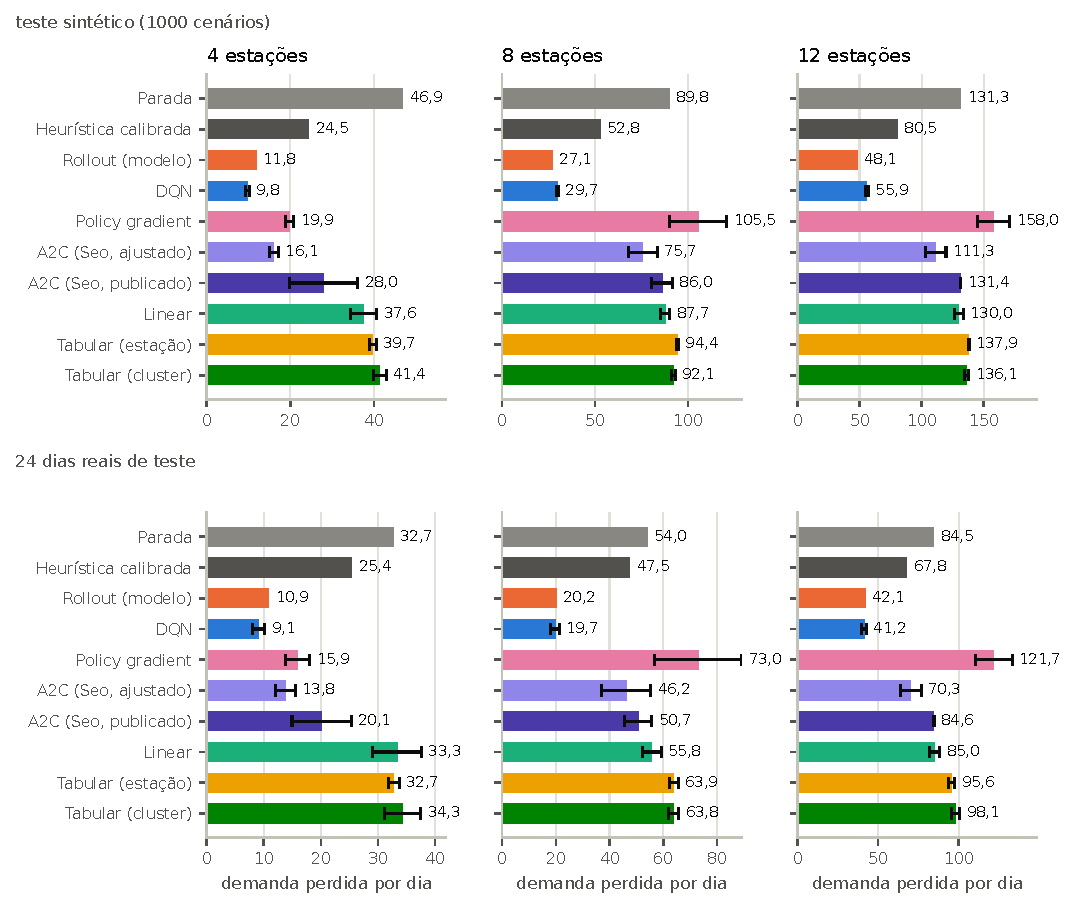
\includegraphics[width=\textwidth]{fig_principal.pdf}
\caption{Demanda perdida por dia (menor \'e melhor). Barras de erro: IC95\% sobre 10 sementes de treino (m\'etodos aprendidos). Parada, heur\'istica e
rollout s\~ao determin\'isticos nos cen\'arios compartilhados.}
\label{fig:principal}
\end{figure}

\subsection{DQN, heur\'istica e rollout}
A Figura~\ref{fig:principal} e a Tabela~\ref{tab:resultados} resumem o experimento principal. No teste sint\'etico, o DQN perde \dqnA, \dqnB e \dqnC\ por
dia (4, 8 e 12 esta\c{c}\~oes; IC95\%: [\dqnLoA; \dqnHiA], [\dqnLoB; \dqnHiB], [\dqnLoC; \dqnHiC]), contra \heurA, \heurB e \heurC\ da melhor heur\'istica
calibrada: uma redu\c{c}\~ao de \redA\%, \redB\% e \redC\%, com o DQN melhor em \nMelhorA, \nMelhorB e \nMelhorC de \nSemA sementes. Nos dias reais, a redu\c{c}\~ao \'e de \redRA\%, \redRB\% e
\redRC\% (\heurRA, \heurRB, \heurRC\ para \dqnRA, \dqnRB, \dqnRC).

O \emph{rollout} sobre o modelo, com $h$ e $K$ escolhidos em valida\c{c}\~ao (cabe\c{c}alho: \rollCfg), perde \rollA, \rollB\ e \rollC. A vantagem do DQN sobre ele \'e de \dqnMenosRollA\
[\dqnMenosRollLoA; \dqnMenosRollHiA] com 4 esta\c{c}\~oes, mas negativa com 8 (\dqnMenosRollB\ [\dqnMenosRollLoB; \dqnMenosRollHiB]) e com 12
(\dqnMenosRollC\ [\dqnMenosRollLoC; \dqnMenosRollHiC]) no teste sint\'etico. Nos dias reais, o DQN fica \`a frente ou empata (\dqnRA\ contra \rollRA,
\dqnRB\ contra \rollRB, \dqnRC\ contra \rollRC). O rollout usa o modelo verdadeiro e seu melhor ajuste ainda estava no limite da grade de $(h,K)$:
seus valores s\~ao um limite inferior do que um planejador com o modelo alcan\c{c}a, e ele custa da ordem de segundos por epis\'odio de avalia\c{c}\~ao (medido em m\'aquina compartilhada), enquanto o DQN decide
quase sem custo depois de treinado. O DQN recupera, portanto, a maior parte do ganho de um planejador com modelo, sem acesso a ele.

\begin{table}[t]
\centering\scriptsize
\setlength{\tabcolsep}{3pt}
\resizebox{\textwidth}{!}{\begin{tabular}{lrrrrrr}
\toprule
& \multicolumn{3}{c}{Teste sintético} & \multicolumn{3}{c}{24 dias reais} \\
\cmidrule(lr){2-4}\cmidrule(lr){5-7}
Método & 4 est. & 8 est. & 12 est. & 4 est. & 8 est. & 12 est. \\
\midrule
Parada & 46,9 & 89,8 & 131,3 & 32,7 & 54,0 & 84,5 \\
Heurística calibrada & 24,5 & 52,8 & 80,5 & 25,4 & 47,5 & 67,8 \\
Rollout (modelo) & 11,8 & 27,1 & 48,1 & 10,9 & 20,2 & 42,1 \\
DQN & 9,8 [9,4; 10,2] & 29,7 [29,0; 30,3] & 55,9 [54,7; 57,1] & 9,1 [8,0; 10,2] & 19,7 [18,2; 21,2] & 41,2 [39,7; 42,8] \\
Policy gradient & 19,9 [18,9; 20,8] & 105,5 [90,1; 120,8] & 158,0 [144,9; 171,0] & 15,9 [13,8; 18,1] & 73,0 [56,9; 89,1] & 121,7 [110,3; 133,1] \\
A2C (Seo et al., publicado) & 28,0 [19,8; 36,2] & 86,0 [80,3; 91,7] & 131,4 [131,3; 131,4] & 20,1 [14,9; 25,3] & 50,7 [45,7; 55,8] & 84,6 [84,5; 84,8] \\
Linear & 37,6 [34,5; 40,7] & 87,7 [85,3; 90,2] & 130,0 [126,6; 133,4] & 33,3 [29,1; 37,6] & 55,8 [52,3; 59,2] & 85,0 [81,7; 88,2] \\
Tabular (estação) & 39,7 [38,9; 40,5] & 94,4 [93,9; 94,9] & 137,9 [137,8; 138,1] & 32,7 [31,8; 33,7] & 63,9 [62,3; 65,5] & 95,6 [93,6; 97,6] \\
Tabular (cluster) & 41,4 [39,8; 42,9] & 92,1 [91,2; 93,0] & 136,1 [134,3; 137,8] & 34,3 [31,2; 37,5] & 63,8 [61,9; 65,8] & 98,1 [95,5; 100,8] \\
\bottomrule
\end{tabular}
}
\caption{Demanda perdida por dia: m\'edia [IC95\% sobre sementes]. Gerada automaticamente dos arquivos de execu\c{c}\~ao.}
\label{tab:resultados}
\end{table}

\subsection{Representa\c{c}\~ao e m\'etodos da literatura}
Tabulares e linear n\~ao superam a heur\'istica em nenhuma escala, mesmo com 16 configura\c{c}\~oes por m\'etodo; em 8 e 12 esta\c{c}\~oes ficam pr\'oximos
ou pior que a pol\'itica parada (\stayB\ e \stayC). O \emph{policy gradient} \'e inst\'avel (desvio-padr\~ao entre sementes de \pgSdB\ e \pgSdC\ em 8 e 12 esta\c{c}\~oes) e s\'o
supera a heur\'istica em 4 esta\c{c}\~oes (\pgA\ contra \heurA, contraste explorat\'orio). O A2C adaptado de \citet{seo2022}, com os hiperpar\^ametros
publicados, perde \acaA, \acaB\ e \acaC\ por dia: colapsa a entropia em cerca de 30 mil passos e termina pr\'oximo da pol\'itica parada com 8 e 12
esta\c{c}\~oes. Ajustado com o mesmo or\c{c}amento dos demais aprendizes (todas as configura\c{c}\~oes escolhidas t\^em b\^onus de entropia), ele passa a perder
\acaTA, \acaTB\ e \acaTC: supera a heur\'istica apenas com 4 esta\c{c}\~oes, fica entre a parada e a heur\'istica com 8 e 12, e fica atr\'as do DQN nas tr\^es escalas.
Isso caracteriza uma adapta\c{c}\~ao (outro simulador, estado e passo de decis\~ao), n\~ao uma falha do m\'etodo original.

\subsection{Efeito da busca de hiperpar\^ametros}\label{sec:busca}
Estender a busca de 8 para 16 configura\c{c}\~oes reduziu a demanda perdida do DQN em \ganhoBuscaA, \ganhoBuscaB\ e \ganhoBuscaC\ (de \dqnOrigA, \dqnOrigB,
\dqnOrigC\ para \dqnA, \dqnB, \dqnC), enquanto em valida\c{c}\~ao o ganho havia sido de \valGanhoA, \valGanhoB\ e \valGanhoC: a escolha por valida\c{c}\~ao superestima o ganho de teste. Para o \emph{policy gradient}, a escolha com duas
sementes de ajuste foi ruidosa: a configura\c{c}\~ao nova melhorou muito com 4 esta\c{c}\~oes e piorou com 12. A Figura~\ref{fig:busca} mostra o efeito
por m\'etodo.

\begin{figure}[t]
\centering
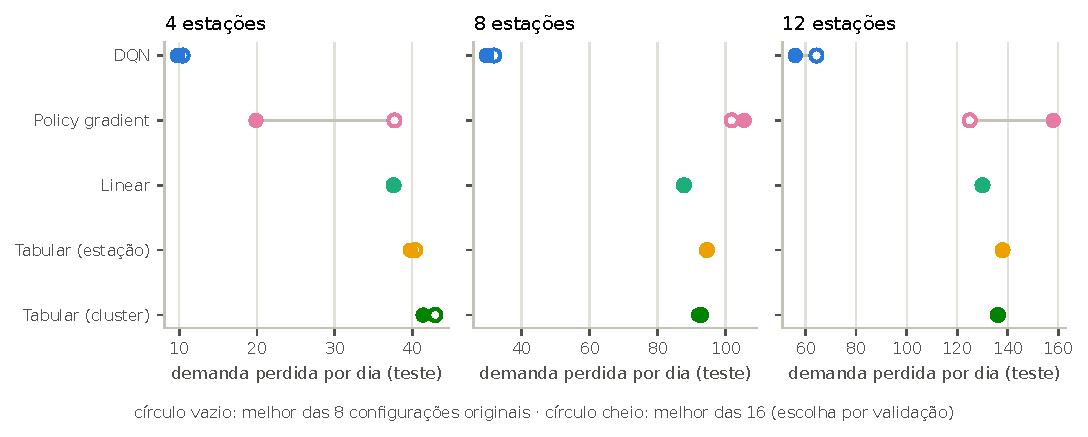
\includegraphics[width=\textwidth]{fig_busca.pdf}
\caption{Efeito de estender a busca de 8 para 16 configura\c{c}\~oes (teste, m\'edia de 10 sementes).}
\label{fig:busca}
\end{figure}

\subsection{Abla\c{c}\~ao do DQN}
Com diferen\c{c}as pareadas por semente (Figura~\ref{fig:ablacao}), remover o \emph{replay} piora o resultado em \ablReplayA\ (4 esta\c{c}\~oes) e
\ablReplayC\ (12), e o agente deixa de aprender em 12 esta\c{c}\~oes. A rede-alvo (\ablAlvoA\ e \ablAlvoC) e o Double DQN (\ablDoubleA\ e \ablDoubleC)
n\~ao apresentam efeito detect\'avel. Apenas o \emph{replay} \'e comprovadamente necess\'ario; a variante sem \emph{replay} faz uma atualiza\c{c}\~ao por
transi\c{c}\~ao com lote 1, o que confunde o \emph{replay} com o n\'umero e o tamanho das atualiza\c{c}\~oes.

\begin{figure}[t]
\centering
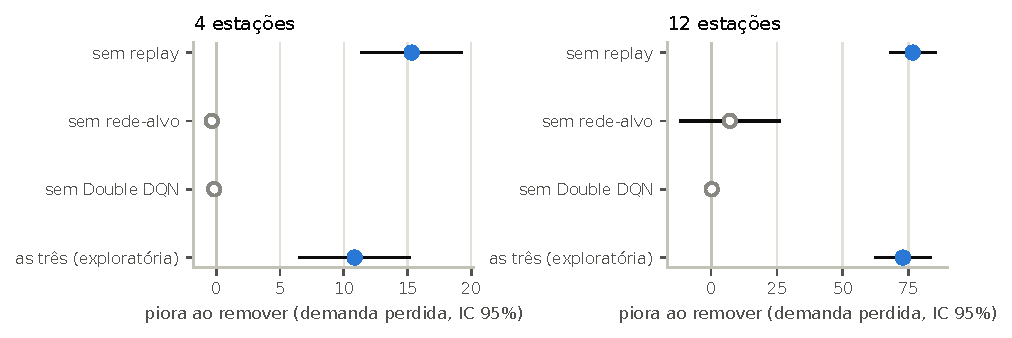
\includegraphics[width=0.85\textwidth]{fig_ablacao.pdf}
\caption{Piora da demanda perdida ao remover cada componente do DQN (diferen\c{c}a pareada por semente, IC95\%). C\'irculo cheio: IC exclui zero.}
\label{fig:ablacao}
\end{figure}

\subsection{Sensibilidade do simulador}
Variamos a demanda em $\times 0{,}5$, $0{,}75$, $1{,}5$ e o tipo de dia (fim de semana), mantendo para os aprendizes a configura\c{c}\~ao escolhida
com demanda $\times 1$ (sem reajuste) e recalibrando a heur\'istica em cada variante, com 5 sementes (Figura~\ref{fig:sens}). Em 4 esta\c{c}\~oes o DQN
supera a heur\'istica em todas as variantes calibradas. Com 12 esta\c{c}\~oes, a vantagem se mant\'em a partir de $\times 0{,}75$, mas com demanda
$\times 0{,}5$ o DQN \'e significativamente pior (\sensKmeioC\ [\sensKmeioCLo; \sensKmeioCHi]) e no fim de semana n\~ao h\'a diferen\c{c}a
detect\'avel (\sensFdsC\ [\sensFdsCLo; \sensFdsCHi]). Como a assimetria (aprendiz sem reajuste contra heur\'istica recalibrada) favorece a
heur\'istica, reajustamos o DQN nessas duas variantes (as mesmas 16 configura\c{c}\~oes, escolha por valida\c{c}\~ao, 5 sementes): o reajuste n\~ao altera
detectavelmente o DQN (\sensKmeioDelta\ [\sensKmeioDeltaLo; \sensKmeioDeltaHi] com demanda $\times 0{,}5$ e \sensFdsDelta\ [\sensFdsDeltaLo; \sensFdsDeltaHi] no
fim de semana) e a diferen\c{c}a para a heur\'istica passa a \sensKmeioRtC\ [\sensKmeioRtCLo; \sensKmeioRtCHi] e \sensFdsRtC\ [\sensFdsRtCLo; \sensFdsRtCHi],
ambas com IC incluindo zero (losangos na Figura~\ref{fig:sens}). Nesses dois regimes, portanto, n\~ao h\'a evid\^encia de vantagem do DQN, e a configura\c{c}\~ao
escolhida com demanda $\times 1$ n\~ao explica a perda sozinha; n\~ao se exclui que alguma configura\c{c}\~ao fora das 16 testadas o recupere.

\begin{figure}[t]
\centering
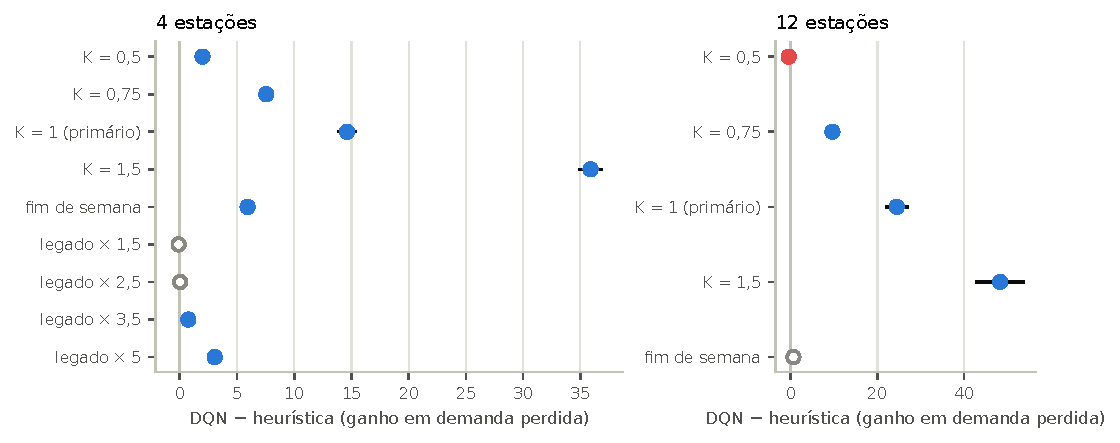
\includegraphics[width=\textwidth]{fig_sensibilidade.pdf}
\caption{DQN $-$ heur\'istica por variante do simulador (5 sementes, IC95\%). Azul: DQN melhor; vermelho: pior; vazio: IC inclui zero. C\'irculo: configura\c{c}\~ao do P1; losango (apenas nas duas variantes de 12 esta\c{c}\~oes em que a conclus\~ao mudou): DQN reajustado na variante.}
\label{fig:sens}
\end{figure}

\section{Limita\c{c}\~oes}\label{sec:lim}
O simulador n\~ao tem roteamento nem tempo de viagem, e o estudo usa um \'unico ve\'iculo; os resultados n\~ao se estendem a frotas ou a rotas reais. A
ocupa\c{c}\~ao inicial dos dias reais \'e desconhecida, e o modelo de Poisson superestima a dificuldade em 30--40\% em rela\c{c}\~ao aos dias reais. O
\emph{rollout} usa o modelo verdadeiro. O A2C \'e uma adapta\c{c}\~ao; a escolha de suas configura\c{c}\~oes usa apenas duas sementes de ajuste. A sensibilidade usa 5 sementes e n\~ao reajusta os aprendizes, exceto o DQN nas duas variantes de 12 esta\c{c}\~oes em que a conclus\~ao mudou. O teto de lote (\emph{batch}) de 256 do DQN \'e imposto por custo; uma verifica\c{c}\~ao com 512 e duas sementes n\~ao mostrou ganho consistente, mas n\~ao exclui um ganho pequeno com 12 esta\c{c}\~oes. Nenhuma
das conclus\~oes foi validada em dados brasileiros ainda. Os resultados preliminares que eram nossa base de partida tinham defeitos (uma semente, escolha
e teste na mesma amostra, heur\'isticas n\~ao calibradas, DQN mal treinado); n\~ao os usamos.

\section{Conclus\~ao}
Em inst\^ancias calibradas com viagens reais, uma rede neural com DQN reduz a demanda perdida em \redA\%, \redB\% e \redC\% (4, 8 e 12 esta\c{c}\~oes) em rela\c{c}\~ao a uma heur\'istica
bem calibrada, e o resultado se mant\'em em dias reais; por\'em, um planejador com o modelo verdadeiro o supera no teste sint\'etico com
8 e 12 esta\c{c}\~oes, e a vantagem n\~ao \'e robusta a demanda baixa com 12 esta\c{c}\~oes. O \emph{replay} \'e o \'unico componente comprovadamente
necess\'ario, e representa\c{c}\~oes simples n\~ao bastam. Trabalhos futuros: roteamento e frota, o estudo de caso com dados brasileiros
(\pend{Tembici}) e um baseline de planejamento mais forte (mais futuros e horizonte maiores).

\bibliographystyle{plainnat}
\bibliography{refs}
\end{document}
